\documentclass{standalone}
\usepackage{tikz}
\usepackage{pgfplots}
\pgfplotsset{compat=newest}
\usepackage{mathptmx}
\usepackage{varwidth}
\usepackage{enumitem}
\usetikzlibrary{calc,patterns,decorations.pathmorphing,decorations.markings,matrix,fit,decorations.pathreplacing,arrows.meta,automata,positioning,shapes,chains,spy}
\usetikzlibrary{intersections,through,backgrounds}
\usetikzlibrary{shadows,fadings}
% \usepackage[active,tightpage,pdftex]{preview}
% \PreviewEnvironment{tikzpicture}
\definecolor{trainingColor}{HTML}{D23AD0}
\definecolor{learningColor}{HTML}{833EC3}
\definecolor{hypothesisColor}{HTML}{2B6BD1}
\definecolor{predictorsColor}{HTML}{F45E30}
\definecolor{targetsColor}{HTML}{FED02F}
\begin{document}\large
  \centerline{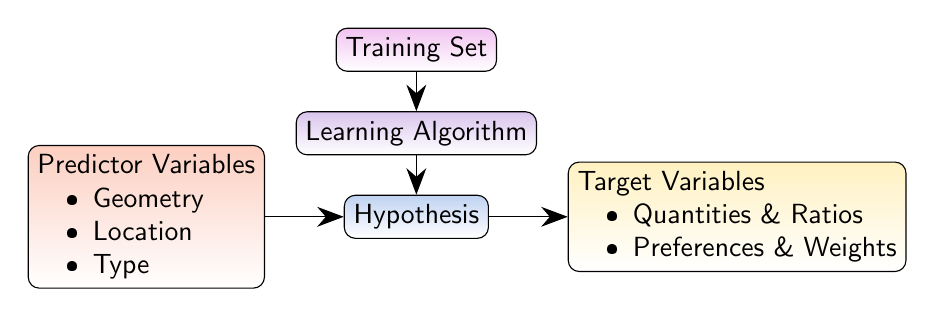
\begin{tikzpicture}[%
    >={Stealth[scale=2.0]},align=center,every node/.style={font=\sffamily}]
    \tikzstyle{state}=[text centered,node distance=0.5cm,%
      rectangle,rounded corners,fill=white,draw=black,%
      minimum width=1.0cm,minimum height=0.45cm]
    \tikzstyle{io}=[text centered,node distance=1.0cm,%
      rectangle,rounded corners,fill=white,draw=black,%
      minimum width=1.0cm,minimum height=0.45cm]
    % All state styles
    \tikzstyle{training}=[state,top color=trainingColor!30]
    \tikzstyle{learning}=[state,top color=learningColor!30]
    \tikzstyle{hypothesis}=[state,top color=hypothesisColor!30]
    \tikzstyle{predictors}=[io,top color=predictorsColor!30]
    \tikzstyle{targets}=[io,top color=targetsColor!30]
    % All states
    \node (training) [training]                          {Training Set};
    \node (learning) [learning,below=of training]        {Learning Algorithm};
    \node (hypothesis) [hypothesis,below=of learning]    {Hypothesis};
    \node (predictors) [predictors,left=of hypothesis]
          {%
            \makebox{%
              \begin{varwidth}{\linewidth}
                Predictor Variables
                \begin{itemize}[noitemsep,topsep=0pt,parsep=0pt,partopsep=0pt,leftmargin=2em]
                \item Geometry
                \item Location
                \item Type
                \end{itemize}\end{varwidth}}};
    \node (targets) [targets,right=of hypothesis]
          {%
            \makebox{%
              \begin{varwidth}{\linewidth}
                Target Variables
                \begin{itemize}[noitemsep,topsep=0pt,parsep=0pt,partopsep=0pt,leftmargin=2em]
                \item Quantities \& Ratios
                \item Preferences \& Weights
                \end{itemize}\end{varwidth}}};
    % Edges
    \draw [->] (training) -- (learning);
    \draw [->] (learning) -- (hypothesis);
    \draw [->] (hypothesis) -- (targets);
    \draw [->] (predictors) -- (hypothesis);
  \end{tikzpicture}}
\end{document}
